
\section{Gestione dei file WAVE}
La gestione dei file audio è affidata alla definizione di moduli detti
\textit{porte}, allo scopo di creare un livello di astrazione sulle informazioni
multimediali contenute al livello di File System.
In questo modo le informazioni multimediali ottenute possono essere agevolmente
processate verso il \textit{conference bridge} che veicola le informazioni
multimediali in entrata od in uscita alla chiamata VoIP che si verrà ad instaurare.
Ogni porta contiene inoltre le informazioni dello stream multimediale in
entrata ed in uscita dalla stessa.

Guardando ora alla funzione \texttt{\small app\_init} definita
all'interno del file \texttt{\small pjsua\_app.c}, dalla quale si inizia l'esecuzione
effettiva dell'applicazione, otteniamo come venga predisposta la \textit{conference}:
\begin{bash}[mathescape=true]
app_init() [pjsua_app.c]
$\drsh$ pjsua_init() [pjsua_core.c]
  $\drsh$ pjsua_media_subsys_init() [pjsua_media.c]
    $\drsh$ pjsua_aud_subsys_init [pjsua_aud.c]
      $\drsh$ pjmedia_conf_create() [conference.c]
\end{bash}

Questa procedura tuttavia si differenzia dall'inizializzazione della porta della
conferenza, che avviene all'apertura del file:
\begin{bash}[mathescape=true]
app_init() [pjsua_app.c]
$\drsh$ pjsua_player_create() [pjsua_aud.c]
  $\drsh$ pjmedia_conf_add_port() [conference.c]
    $\drsh$ create_conf_port()
\end{bash}
In questo punto avviene l'effettiva inizializzazione della porta di conferenza,
grazie alle informazioni ottenibili dalla porta audio precedentemente 
aperta sul file audio, e l'inizializzazione dei buffer per la ricezione dei
dati dalla porta di conferenza, o in uscita verso la stessa. Tuttavia nemmeno
qui si ottengono le informazioni sulle caratteristiche del file 
audio. 

L'inizializzazione delle informazioni dalla porta audio avviene nella funzione
\texttt{\small pjmedia\_wav\_player\_port\_create}, richiamata direttamente dalla
funzione \texttt{\small pjsua\_player\_create()}, prima dell'aggiunta della porta
ottenuta alla porta di conferenza in \texttt{\small pjmedia\_conf\_add\_port()}.
All'interno della funzione suddetta, dopo aver aperto una porta sul file audio
ed aver acceduto al file in lettura, si ottengono le informazioni dallo
header del file WAVE, che vengono utilizzati nella funzione 
\texttt{\small pjmedia\_port\_info\_init} per impostare i valori di default della
porta. 

\subsection{Premessa: struttura di un file WAVE}
\begin{figure}[thp]
\centering
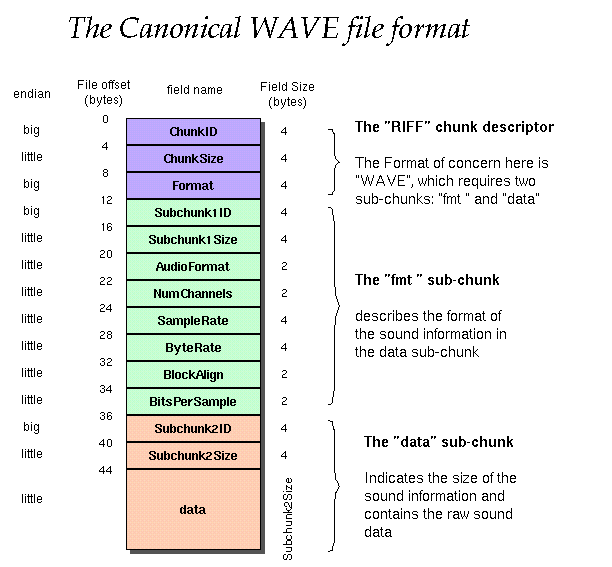
\includegraphics[scale=0.65]{img/wav-sound-format.png}
\caption{Struttura di un file WAVE. \url{http://math2033.uark.edu/wiki/images/4/45/Wav-sound-format.gif}}
\label{fig:imgwave}
\end{figure}
Presento qui un'introduzione sulla struttura di un file WAVE (contrazione di 
\textit{WAVEform audio file format}): tale formato audio è costituito principalmente 
da vari \textit{chunk}  caratterizzati da uno \textit{header} iniziale, e da dati che 
seguono. La struttura standard di un file WAVE è presentata in  Figura
\vref{fig:imgwave}, dalla quale si può evincere come principalmente possano
esistere 3 \textit{chunk} chiamati \textit{RIFF}, \textit{format} e \textit{data}:
\begin{description}
\item[RIFF] Questo primo \textit{chunk} contiene uno header che contraddistingue
	tale file come WAVE: in particolare il primo ed il terzo campo assumono
	il valore rispettivamente di \texttt{\small RIFF} e \texttt{\small WAVE}, mentre
	il secondo indica la dimensione delle informazioni inglobate dopo il terzo
	campo.
\item[Format] Questo secondo \textit{chunk} e accomunato a tutti gli altri, escluso
	il precedente, dai campi \texttt{\small ChunkID} e \texttt{\small ChunkDataSize}.
	I campi rimanenti caratterizzano il tipo di compressione (es. \texttt{PCM} - ovvero
	non compresso, \textit{GSM}, \textit{MPEG}), i canali audio utilizzati, il numero
	di campionamenti al secondo (valore indipendente dal numero
	dei canali), quanti \textit{bytes} devono essere riprodotti al secondo per 
	riprodurre l'audio contenuto ($ByteRate = SampleRate \cdot BlockAlign$),
	la dimensione di ciascun campionamento ($BlockAlign = \frac{bpsample}{8} \cdot NumChannels$),
	il numero dei \textit{byte} utilizzato per definire ciascun campionamento e 
	il numero di \textit{byte} addizionali che segue.
\item[Data] Questo terzo  \textit{chunk} contiene le informazioni digitalizzate dell'audio.
\end{description}

Possiamo osservare un esempio di come ottenere queste informazioni tramite il
file fornito nella Sottosezione \vref{subsec:appreadwave}, che è stato utile
ai fini di individuare, all'interno del codice di \textit{pjmedia}, l'ottenimento
delle informazioni dal file WAVE.



